\newcommand{\splw}{\textwidth}
\newcommand{\splh}{\splw}

% \newcommand{\splnrverticallines}{11}
% \newcommand{\splverticalinterval}{0.08333} % 1 / (splnrverticallines + 1)
\newcommand{\splnrverticallines}{19}
\newcommand{\splverticalinterval}{0.05} % 1 / (splnrverticallines + 1)

% \newcommand{\splnrhorizontallines}{11}
% \newcommand{\splhorizontalinterval}{0.08333}
\newcommand{\splnrhorizontallines}{19}
\newcommand{\splhorizontalinterval}{0.05}

\begin{tikzpicture}[
    cline/.style = {very thick, color-one},
]
    \begin{scope}
        \node[anchor=south west,inner sep=0] at (0,0) {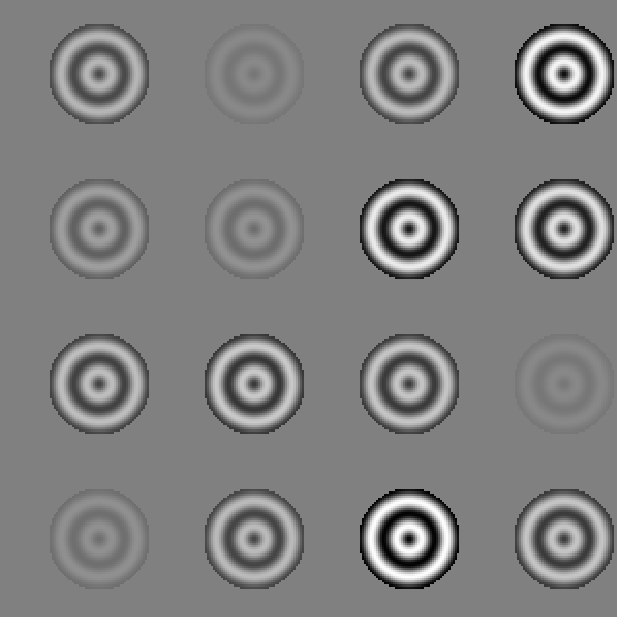
\includegraphics[width=\splw]{src/assets/images/stimulus-patch-lattice.png}};
        
        % vertical
        \foreach \i in {1, 2, ..., \splnrverticallines}{
            \draw[cline] (\i * \splverticalinterval * \splw, 0) -- (\i * \splverticalinterval * \splw, \splh) {};
        }
        
        % horizontal
        \foreach \i in {1, 2, ..., \splnrverticallines}{
            \draw[cline] (0, \i * \splhorizontalinterval * \splh) -- (\splw, \i * \splhorizontalinterval * \splh) {};
        }

    \end{scope}
\end{tikzpicture}